\documentclass[tikz,border=5pt]{standalone}
\usepackage{luatexja}
\usepackage[hiragino-pron]{luatexja-preset}
\usepackage{amsmath,amssymb}
\usetikzlibrary{arrows.meta,patterns,calc}

\begin{document}
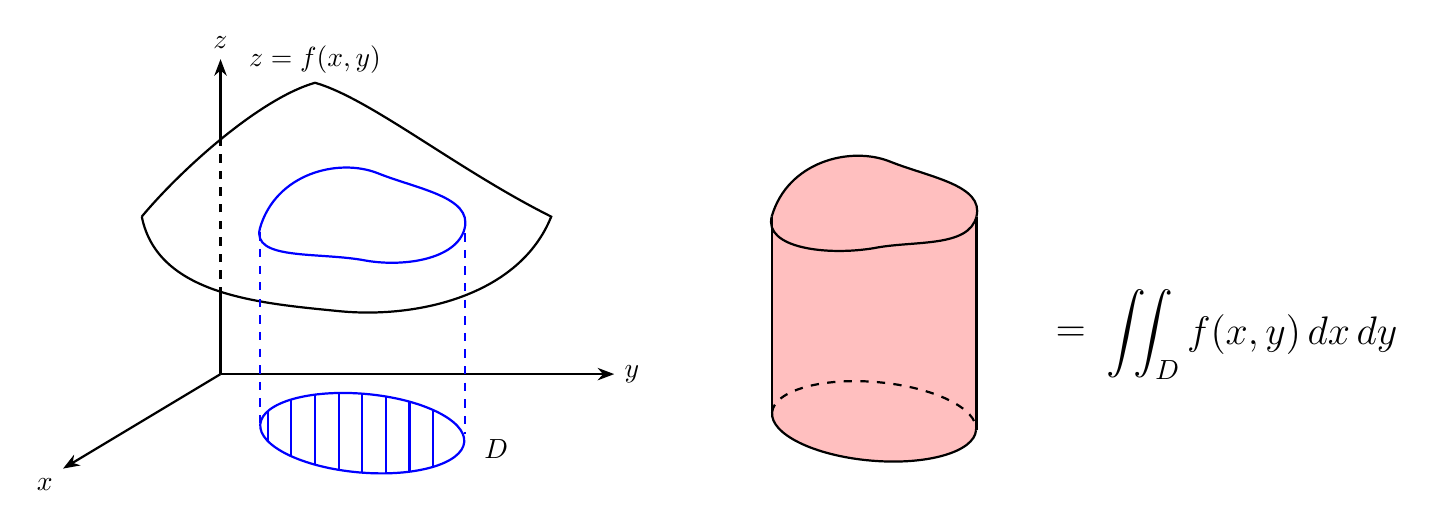
\begin{tikzpicture}

% === Left: 3D surface z=f(x,y) over domain D ===
\begin{scope}[shift={(0,0)}]

% Oblique projection: x-axis goes right-forward, y-axis goes left, z goes up
% Origin at (-1, 0.8)
\coordinate (O) at (-1,0.8);

% Axes
% z-axis: split into solid (below surface), dashed (behind surface), solid (above surface)
\draw[thick] (O) -- ++(0,1.0);           % below surface
\draw[thick, dashed] (-1,1.8) -- (-1,3.8);  % behind surface
\draw[-{Stealth[length=6pt]}, thick] (-1,3.8) -- ++(0,1.0) node[above] {$z$}; % above surface
\draw[-{Stealth[length=6pt]}, thick] (O) -- ++(5.0,0) node[right] {$y$};
\draw[-{Stealth[length=6pt]}, thick] (O) -- ++(-2.0,-1.2) node[below left] {$x$};

% --- Domain D on xy-plane (blue hatched ellipse) ---
% Center of D in projected coordinates
\coordinate (Dc) at (0.8,0.05);

% Ellipse for D
\draw[blue, thick] (Dc) ellipse [x radius=1.3, y radius=0.5, rotate=-5];

% Hatching inside D
\clip (Dc) ellipse [x radius=1.3, y radius=0.5, rotate=-5];
\foreach \i in {-1.2,-0.9,...,1.2} {
  \draw[blue, thick] ($(Dc)+(\i,-0.6)$) -- ($(Dc)+(\i,0.6)$);
}
% Reset clip
\begin{scope}
\end{scope}

\end{scope}

% Re-draw without clip
\begin{scope}[shift={(0,0)}]
\coordinate (O) at (-1,0.8);
\coordinate (Dc) at (0.8,0.05);

% D label
\node at ($(Dc)+(1.7,-0.2)$) {$D$};

% --- Surface z = f(x,y) (flat dome with sharp corners, top pointed) ---
\draw[thick]
  (-2.0,2.8)
  .. controls (-1.5,3.4) and (-0.5,4.3) .. (0.2,4.5)
  .. controls (0.9,4.3) and (2.0,3.4) .. (3.2,2.8)
  -- (3.2,2.8)
  .. controls (2.8,1.8) and (1.5,1.5) .. (0.5,1.6)
  -- (0.5,1.6)
  .. controls (-0.5,1.7) and (-1.8,1.8) .. (-2.0,2.8);

% z = f(x,y) label
\node[above] at (0.2,4.5) {$z = f(x,y)$};

% --- Blue curve on surface (directly above D, slightly warped) ---
\draw[blue, thick]
  (-0.5,2.65) .. controls (-0.3,3.35) and (0.5,3.55) .. (1.0,3.35)
  .. controls (1.5,3.15) and (2.2,3.05) .. (2.1,2.65)
  .. controls (2.0,2.25) and (1.3,2.15) .. (0.8,2.25)
  .. controls (0.2,2.35) and (-0.6,2.25) .. (-0.5,2.65);

% --- Dashed vertical lines connecting D to surface (left and right of ellipse) ---
\draw[blue, dashed, thick] (-0.5,2.60) -- (-0.5,0.15);
\draw[blue, dashed, thick] (2.1,2.80) -- (2.1,0.04);

\end{scope}

% === Right: Volume with exact same shape as left blue region ===
\begin{scope}[shift={(6.5,0)}]

% Pink fill: single unified fill
% Bottom ellipse
\begin{scope}[shift={(0.8,0.2)}, rotate=-5]
  \fill[pink] (0,0) ellipse [x radius=1.3, y radius=0.5];
\end{scope}
% Side walls + top as single path
\fill[pink]
  (-0.5,0.31) -- (-0.5,2.8)
  .. controls (-0.3,3.5) and (0.5,3.7) .. (1.0,3.5)
  .. controls (1.5,3.3) and (2.2,3.2) .. (2.1,2.8)
  -- (2.1,0.09) -- cycle;
\fill[pink]
  (-0.5,0.31) -- (-0.5,2.8)
  .. controls (-0.6,2.4) and (0.2,2.3) .. (0.8,2.4)
  .. controls (1.3,2.5) and (2.0,2.4) .. (2.1,2.8)
  -- (2.1,0.09) -- cycle;

% Bottom ellipse stroke
\begin{scope}[shift={(0.8,0.2)}, rotate=-5]
  % Back half (dashed)
  \draw[thick, dashed] (180:1.3 and 0.5) arc[x radius=1.3, y radius=0.5, start angle=180, end angle=0];
  % Front half (solid)
  \draw[thick] (180:1.3 and 0.5) arc[x radius=1.3, y radius=0.5, start angle=180, end angle=360];
\end{scope}

% Top warped curve (exact same as left blue curve)
\draw[thick]
  (-0.5,2.8) .. controls (-0.3,3.5) and (0.5,3.7) .. (1.0,3.5)
  .. controls (1.5,3.3) and (2.2,3.2) .. (2.1,2.8);
\draw[thick]
  (-0.5,2.8) .. controls (-0.6,2.4) and (0.2,2.3) .. (0.8,2.4)
  .. controls (1.3,2.5) and (2.0,2.4) .. (2.1,2.8);

% Side walls
\draw[thick] (-0.5,0.31) -- (-0.5,2.8);
\draw[thick] (2.1,0.09) -- (2.1,2.8);

% Equals sign and integral
\node at (3.3,1.3) {\Large $=$};
\node at (5.6,1.3) {\Large $\displaystyle\iint_D f(x,y)\,dx\,dy$};

\end{scope}

\end{tikzpicture}
\end{document}
